\documentclass{article}
\usepackage{amsmath,amsfonts,amsthm,amssymb,amsopn,bm}
\usepackage[margin=.9in]{geometry}
\usepackage{graphicx}
\usepackage{url}
\usepackage[usenames,dvipsnames]{color}
\usepackage{fancyhdr}
\usepackage{multirow}
\usepackage{listings}
\usepackage{hyperref}

\definecolor{keywords}{RGB}{255,0,90}
\definecolor{comments}{RGB}{0,0,113}
\definecolor{red}{RGB}{160,0,0}
\definecolor{green}{RGB}{0,150,0}
 
\lstset{language=Python, 
        basicstyle=\ttfamily\tiny, 
        keywordstyle=\color{keywords},
        commentstyle=\color{comments},
        stringstyle=\color{red},
        showstringspaces=false}

\newcommand{\field}[1]{\mathbb{#1}}
\newcommand{\1}{\mathbf{1}}
\newcommand{\E}{\mathbb{E}} 
\newcommand{\Z}{\mathbb{Z}} 
\renewcommand{\P}{\mathbb{P}}
\newcommand{\R}{\field{R}} % real domain
% \newcommand{\C}{\field{C}} % complex domain
\newcommand{\F}{\field{F}} % functional domain
\newcommand{\T}{^{\textrm T}} % transpose
\def\diag{\text{diag}}

%% operator in linear algebra, functional analysis
\newcommand{\inner}[2]{#1\cdot #2}
\newcommand{\norm}[1]{\left\|#1\right\|}
\newcommand{\twonorm}[1]{\|#1\|_2^2}
% operator in functios, maps such as M: domain1 --> domain 2
\newcommand{\Map}[1]{\mathcal{#1}}
\renewcommand{\theenumi}{\alph{enumi}} 

\newcommand{\Perp}{\perp \! \! \! \perp}

\newcommand\independent{\protect\mathpalette{\protect\independenT}{\perp}}
\def\independenT#1#2{\mathrel{\rlap{$#1#2$}\mkern2mu{#1#2}}}
\newcommand{\vct}[1]{\boldsymbol{#1}} % vector
\newcommand{\mat}[1]{\boldsymbol{#1}} % matrix
\newcommand{\cst}[1]{\mathsf{#1}} % constant
\newcommand{\ProbOpr}[1]{\mathbb{#1}}
\newcommand{\points}[1]{\small\textcolor{magenta}{\emph{[#1 points]}} \normalsize}
\date{{}}

\setlength\parindent{0px}

\begin{document}
\title{Homework \#5}
\author{\normalsize{Winter 2020, STATS 509}\\
\normalsize{Dino Bektesevic}}
\maketitle



\section*{Problem 1}
Let $X_1$ and $X_2$ be independent random variables, with means $\mu_1$, $\mu_2$, and variances $\sigma^2_1$ and $\sigma^2_2$ respectively. Further, let $S = (X_1 + X_2)/2$ and $T = (X_1 - X_2)/2$. Find:
\begin{enumerate}
    \item[(a)] E$[S]$ and E$[T]$;

    \begin{align*}
        E[S] &= E[X_1/2 + X_2/2] \\
        &= \frac{1}{2}E[X_1] + \frac{1}{2}E[X_2] \\
        &= \frac{1}{2}\mu_1 + \frac{1}{2}\mu_2 \\
    \end{align*}
    
    \begin{align*}
        E[T] &= E[X_1/2 - X_2/2] \\
        &= \frac{1}{2}E[X_1] - \frac{1}{2}E[X_2] \\
        &= \frac{1}{2}\mu_1 - \frac{1}{2}\mu_2 \\
    \end{align*}
    
    \item[(b)] V$(S)$ and V$(T)$;

    \begin{align*}
        V[S] &= V[X_1/2 + X_2/2] \\
        &= \frac{1}{4}V[X_1] + \frac{1}{4}V[X_2] + \frac{1}{2}Cov(X_1, X_2)\\
        &= \frac{1}{4}\sigma_1 + \frac{1}{4}\sigma_2 \\
    \end{align*}
    
    \begin{align*}
        V[S] &= V[X_1/2 - X_2/2] \\
        &= \frac{1}{4}V[X_1] + \frac{1}{4}V[X_2] - \frac{1}{2}Cov(X_1, X_2)\\
        &= \frac{1}{4}\sigma_1 + \frac{1}{4}\sigma_2 \\
    \end{align*}

    \item[(c)] Cov$(S,T)$;

    \begin{align*}
        Cov(S, T) &= Cov\left(\frac{X_1}{2}+\frac{X_2}{2}, \frac{X_1}{2}-\frac{X_2}{2} \right) \\
        &= \frac{1}{4} Cov(X_1, X_1) - \frac{1}{4} Cov(X_1, X_2) - \frac{1}{4}Cov(X_2, X_1) + \frac{1}{4} Cov(X_2, X_1)\\
        &= \frac{\sigma_1}{4} + \frac{\sigma_2}{4} - \frac{1}{2}Cov(X_1, X_2) \\
        &= \frac{\sigma_1 + \sigma_2}{4}
    \end{align*}

    \item[(d)] Cov$(X_1,S)$, Cov$(X_2,T)$.
    
    $$Cov\left(X_1, \frac{X_1}{2}+\frac{X_2}{2}\right) = \frac{1}{2} Cov(X_1, X_1) =  \frac{\sigma_1}{2} $$
    $$Cov\left(X_2, \frac{X_1}{2}-\frac{X_2}{2}\right) = -\frac{1}{2} Cov(X_2, X_2) =  -\frac{\sigma_2}{2} $$
\end{enumerate}



\newpage
\section*{Problem 2}
Suppose that $X$ is a continuous random variable with support on $\mathbb{R}$. Suppose that the pdf for $X$ is symmetric around a point $t$, so that $f(t-x) = f(t+x)$ for all $x$.
\begin{enumerate}
    \item Find the median of $X$. {\it Hint: use the fact that the pdf integrates to $1$ and then split the integral into two pieces.}
    
    
    \item Find the mean of $X$. {\it Hint: use the fact that $E[X] = t^*$ if and only if $E[X-t^*]=0$. Again split the integral; also see Midterm Qu.3(b)} 
    
    \begin{align*}
        E[X] &= \int_{-\infty}^\infty xf_X dx \\
        &= \int_{-\infty}^t xf(t-x)dx + \int_t^\infty xf(x+t)dx \\
        &= \int_t^\infty xf(t+x)dx + \int_t^\infty xf(x+t)dx \\
        &= 2\int_t^\infty xf(x+t)dx
    \end{align*}
\end{enumerate}



\newpage
\section*{Problem 3}
Consider a continuous random variable with pdf $f_X(x)$ and CDF $F_X(x)$.
\begin{enumerate}
    \item Show that $\int_{-\infty}^t F_X(x) dx = \int_{-\infty}^t f(u) (t-u) du$.\par {\it Hint: recall HW3 Qu.3}
    \item Similarly show that $\int_{t}^\infty (1-F_X(x)) dx = \int_{t}^\infty f(u) (u-t) du$.
\end{enumerate}
Define $h(t) \equiv E|X-t|$; the average absolute value of the prediction error, when using the constant $t$ as a prediction (for all units).
\begin{enumerate}
    \item[(c)] Show that $h(t) =  \int_{-\infty}^t F_X(x) dx + \int_t^\infty(1 - F_X(x))dx$.
    \item[(d)] Using your answer to (c) show that $h(t)$ is minimized when $t$ is a median for $X$. Recall that $m$ is a median for $X$ if $F_X(m) = 0.5$.\par
            {\it Hint: use the Fundamental Theorem of Calculus and your answer to (c).}
\end{enumerate}



\newpage
\section*{Problem 4.} Goldberger Question 6.2



\newpage
\section*{Problem 5.} 

For this question use the following dataset:\par
{\scriptsize \url{http://www.stat.washington.edu/tsr/s509/examples/pres-election-2016-pop-density.csv}}\par
The dataset contains two variables measured in every US county:
\begin{enumerate}
    \item {\tt log10popdens}: the logarithm (base 10) of the population density measured in people per square kilometer;
    \item{\tt logpartyratio}: the natural logarithm of the ratio of the vote share for Hillary Clinton to the vote share for Donald Trump in 2016.
\end{enumerate}
The dataset also contains the county name and the state. Using {\tt R} or a similar package find:
\begin{enumerate}
    \item[(a)] The best linear predictor of {\tt logpartyratio} from  {\tt log10popdens}.
    \item[(b)] The approximate conditional expectation function\par
        E[ {\tt logpartyratio} $|$ {\tt log10popdens} ] by dividing {\tt log10popdens} into 13 bins:
        $$(-2.0,-1.5], (-1.5,-1.0], \ldots ,(4.0,4.5]$$
        and computing the mean in each bin.\par
        {\it Hint: In {\tt R} these are the bins given by the {\tt hist} function.}
    \item[(c)] The conditional expectation function via the loess smoother for\par
        E[ {\tt logpartyratio} $|$ {\tt log10popdens} ]
\end{enumerate}
Construct a scatterplot showing the data together with these three functions. Also provide the code that you used. {\it  See the example code here:}\url{http://www.stat.washington.edu/tsr/s509/examples/edwage.r}

\begin{center}
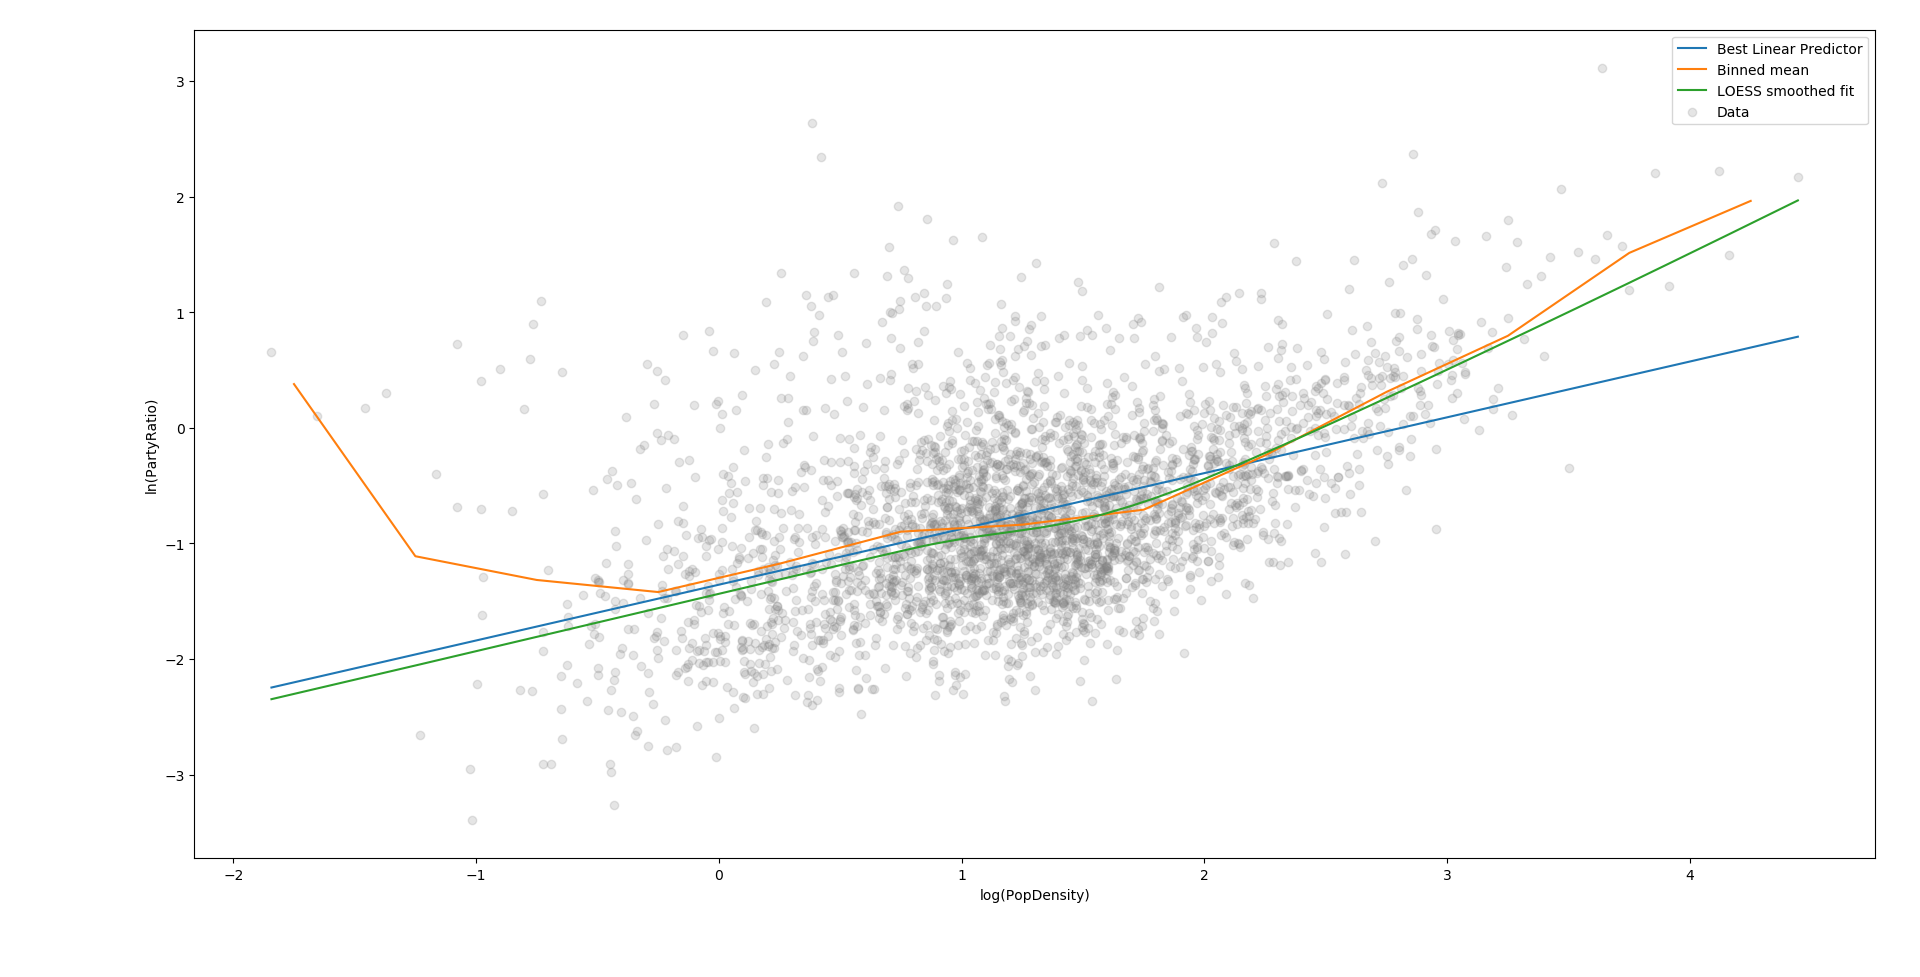
\includegraphics[width=500px]{STATS509/HW5/problem5.png}
\end{center}

\newpage
\lstinputlisting[language=Python]{HW5Code/HW5_DinoBektesevic.py}


\newpage
\section*{Problem 6.}
A population consists of two types, {\it humans} and {\it replicants}. The proportion of replicants is $q$. The height of each type approximately follow normal distributions. Let $N(\mu_H,\sigma^2_H)$ be the distribution of lengths for humans; let $N(\mu_R,\sigma^2_R)$ be the distribution of lengths for replicants.
\begin{enumerate}
    \item Find the mean height of a randomly sampled subject in this population.
    \item Find the variance of the distribution of height for subjects in this population.
\end{enumerate}



\newpage
\section*{Problem 7}
Suppose that $X$ and $Y$ are continuous random variables, with support on $\mathbb{R}^2$.
Suppose that two researchers, Thelma and Louise, wish to predict $Y$ from $X$ using a function of $X$.
\begin{enumerate}
    \item Thelma wishes to use the function $g_T(X)$ that minimizes  the average squared prediction $E[(Y-g_T(X))^2]$. What function will Thelma use? {\it You may justify your answer by quoting results from the Lecture.}
    \item Louise, however, wishes to use the function $g_L(X)$ that minimizes the average absolute error $E[|Y-g_L(X)|]$. What function will Louise choose?  Explain your answer. {\it Hint: Use the law of iterated expectations and Qu.3.}
    \item Suppose that there is a function $r(x)$ such that the conditional density for $Y$ given $X=x$ is symmetric around $r(x)$, so that for all $x$ and $y$, $f(r(x) - y \,|\,x) =  f(r(x)+y \,|\,x)$, what can we say about the functions $g_T(X)$ and $g_L(X)$ used by Thelma and Louise? \par
    {\it Hint: Use Qu.2.}
\end{enumerate}



\newpage
\section*{Problem 8} Suppose a medical test has the following characteristics:
\begin{eqnarray*}
    Pr(\hbox{Test +ve} \mid \hbox{Patient Diseased})&=& 0.99\\
    Pr(\hbox{Test -ve} \mid \hbox{Patient Not Diseased})&=& 0.98
\end{eqnarray*}

\begin{enumerate}
    \item[(a)] Find $Pr(\hbox{Test -ve} \mid $ Patient Diseased $)$ and $Pr(\hbox{Test +ve} \mid$ Patient Not Diseased $)$.
\end{enumerate}

Suppose that 1 in 5,000 people have this disease so $Pr(\hbox{Patient Diseased}) = 0.0002$
\begin{enumerate}
    \item[(b)] Compute $Pr( \hbox{Test +ve} )$. {\it Hint: Find $Pr(\hbox{Test +ve},$ {Patient Diseased}$)$ and $Pr(\hbox{Test +ve},$ {Patient Not Diseased}$)$.}
    \item[(c)] Use Bayes' rule to find $Pr(\hbox{Patient Diseased} |$ {Test +ve}$)$.
    \item[(d)] Give an intuitive explanation for the discrepancy between $Pr($ Patient Diseased $|$ {Test +ve}$)$ and $Pr($ {Test +ve} $|$ Patient Diseased).
\end{enumerate}
\end{document}
